% !TEX encoding = UTF-8 Unicode
\documentclass[screen, aspectratio=169]{beamer}
\usepackage[T1]{fontenc}
%\usepackage[utf8]{inputenc}

% Use the NTNU-temaet for beamer 
% \usetheme[style=ntnu|simple|vertical|horizontal, 
%     language=bm|nn|en, 
%     smalltitle, 
%     city=all|trondheim|alesund|gjovik]{ntnu2017}
\usetheme[style=ntnu,language=en]{ntnu2017}

\usepackage[english]{babel}
\usepackage[style=numeric,backend=biber,natbib=false,sorting=none]{biblatex}

\title[HCI-intro]{Human Computer Interaction}
\subtitle{Trends in HCI}
\author[A. Xamb{\'o}]{Anna Xamb{\'o}}
\institute[NTNU]{Department of Music, NTNU}
\date{October 22, 2019}
%\date{} % To have an empty date

\addbibresource{../hci-lectures.bib} % Add bibliography database

% Set the reference style to numeric.
% See here: http://tex.stackexchange.com/questions/68080/beamer-bibliography-icon
\setbeamertemplate{bibliography item}[text] 

% Set bibliography fonts to a small size.
\renewcommand*{\bibfont}{\footnotesize}

\begin{document}

\begin{frame}
  \titlepage
\end{frame}

% Alternatively, special title page command to get a different background
% \ntnutitlepage

\begin{frame}
\frametitle{Learning Outcomes}
\begin{itemize}
\item Get a sense of the differences between 1st, 2nd, and 3rd wave in HCI.
\item Explore a range of key topics in the HCI discipline.
\item Identify the format of CHI paper writing.
\item Discover the elements in a successful CHI paper submission.
\end{itemize}
\end{frame}
%
\begin{frame}
\frametitle{Preparation: Reading}
\begin{itemize}
\item Watch this video, which explains how the course will work: \url{http://folk.ntnu.no/annax/MCT-videos/VL-2018-10-15-09-01-MCT.mp4}, slides here.
\item Send a summary (1 page max.) of the following article:
\begin{itemize}
\item Being Human Human-Computer Interaction in the Year 2020 \cite{Harper.et.al.2008.being}\\
\url{https://hxd.research.microsoft.com/manage/resources/beinghumana3-1.pdf} 
\end{itemize}
You should pick one subsection (e.g. 1.1 changing computers, 2.2. the end of interface stability, 3.2 extending the research and design cycle) and briefly summarize it reflecting on the present day: (1) give the context of the text,
(2) summarize the subsection, and (3) reflect on the present day.
\end{itemize}
\end{frame}
%
\begin{frame}
\frametitle{Final Assignment (1/2)}
{\small
\begin{itemize}
\item The final assignment of this course will consist in writing a short paper (4 pages long) about the prototype that you built in team and presented during the mini-hackathon of the Physical Computing Workshop.
\item The paper will have both individual parts (written individually) and group parts (written in team). 
\item This final assignment will count 40\% of the total grading of the course, where 50\% will count from your individual contributions and 50\% will count from group contributions.
\item Page about the final assignment on Canvas: \url{https://uio.instructure.com/courses/22318/assignments/28321}
\end{itemize}
}
\end{frame}
%
\begin{frame}
\frametitle{Final Assignment (2/2)}
{\small
The paper structure should have the following sections:
\begin{itemize}
\item Title
\item Abstract (300 words)
\item Introduction (\emph{group})
\item Background (\emph{group})
\item The System (\emph{group})
\item The Performance (\emph{group})
\item Reflective Notes (\emph{individual})
\item Conclusion (\emph{individual})
\end{itemize}
}
\end{frame}
%
\begin{frame}
\frametitle{Class Structure}
\begin{itemize}
\item 10.15-10.45 Presentation course/day. Presentation/lecture of the 1st, 2nd, and 3rd wave in HCI.
\item 10.30-11.00 Discussion about the prep. reading framed in the context of the three waves in HCI.
\item 11.00-11.30 Teamwork: Selection of a paper from the CHI 2019 Best Papers (\url{https://chi2019.acm.org/2019/03/15/chi-2019-best-papers-honourable-mentions/}) and discussion about what is the research question, the approach used to address the research question, the main findings and the main contribution.
\item 11.30-12.00 The teams summarize to the group their selected paper (10 min per group).
\end{itemize}
\end{frame}
%
\begin{frame}
\frametitle{}
\Huge{What is HCI?}
\end{frame}
%
\begin{frame}
\frametitle{What is HCI?}
 \begin{figure}
	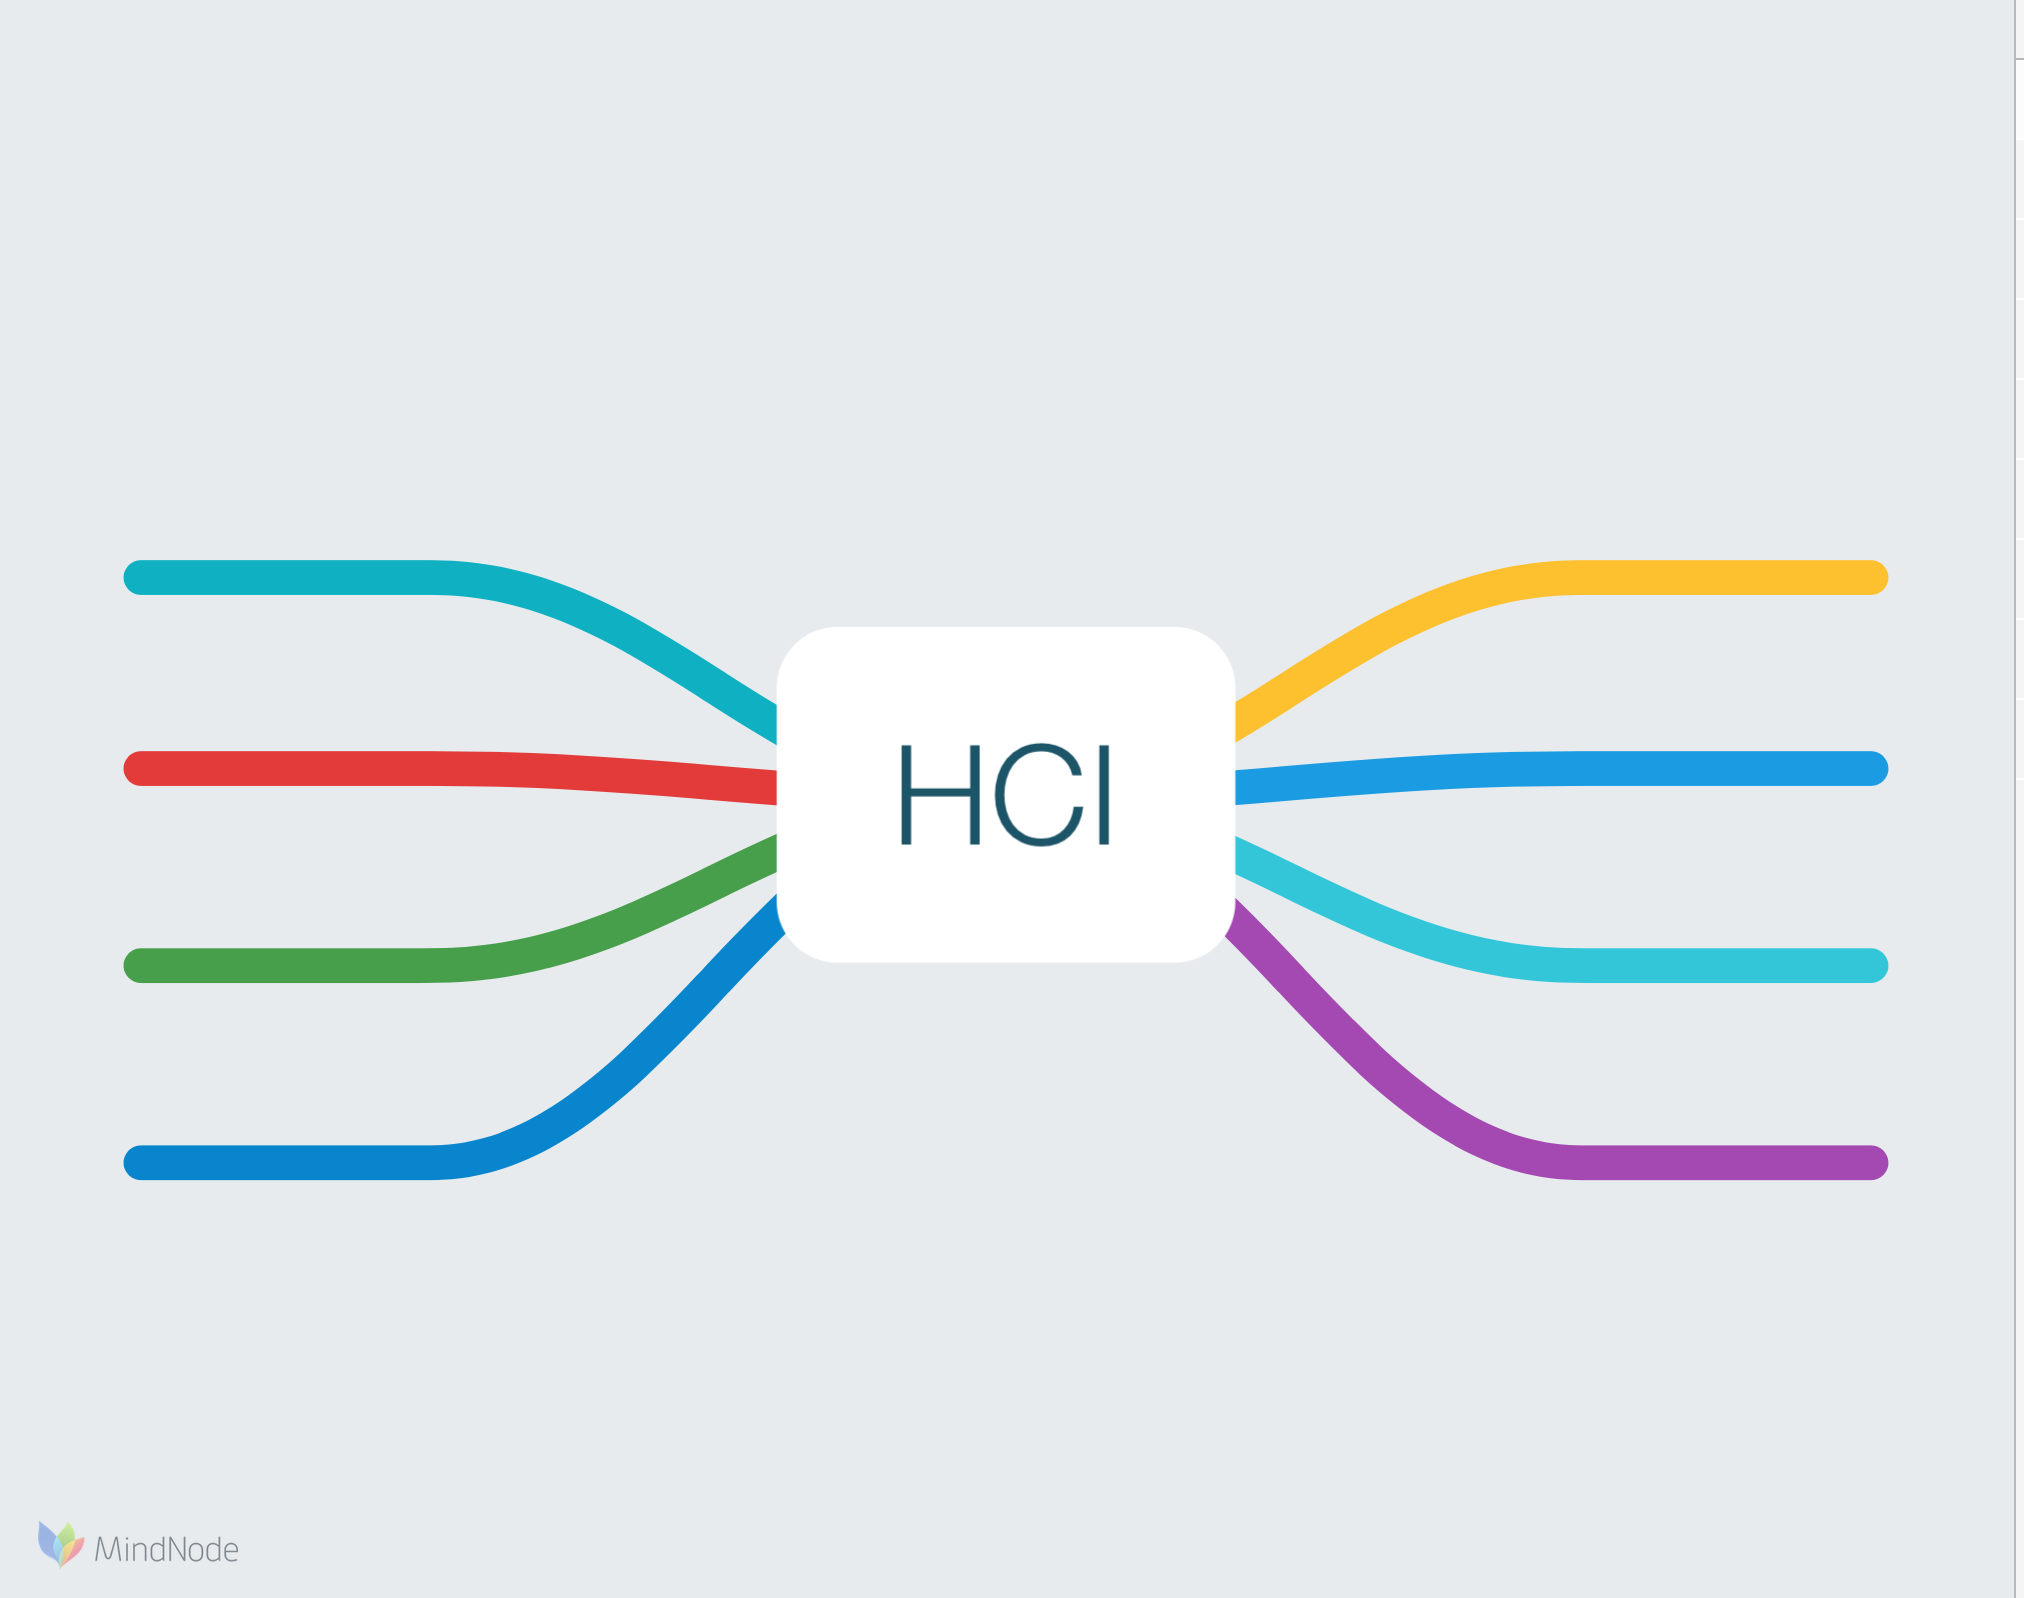
\includegraphics[scale=0.22]{img/HCI-empty-mindmap.png}
    \end{figure}	
\end{frame}
%
\begin{frame}
\frametitle{What is HCI?}
\begin{quote}
Human-computer interaction is a discipline concerned with the design, evaluation and implementation of interactive computing systems for human use and with the study of major phenomena surrounding them. \cite{Hewett.1992.curricula} 
\end{quote}
\begin{itemize}
\item HCI is described as a constantly changing field.
\item \emph{Interaction Design} is concerned with the theory, research, and practice of designing user experiences for all manner of technologies, systems, and products.~\cite{Preece.et.al.2015.ic-book}
\item \emph{Ergonomics and Human Factors} have closely overlapping goals with HCI, being concerned with understanding the interactions among humans and other aspects of a system in order to optimize human well-being and overall system performance.~\cite{Preece.et.al.2015.ic-book}
\end{itemize}
\end{frame}
%
\begin{frame}
\frametitle{What is an HCI course?}
The basic elements of an HCI course can be consulted on the Association for Computing Machinery's Special Interest Group on Computer-Human Interaction (ACM SIGCHI) online statement: 
\begin{quote}
SIGCHI members are involved in the design, implementation, and use of interactive computer-based systems in the broadest sense.\footnote{\url{https://interactions.acm.org/about-sigchi}} 
\end{quote}
A course that includes any of these aspects of interactive systems can be categorized as an HCI course.\\
It has been highlighted that HCI education is an ongoing field that is rapidly and continually changing in order to keep in alignment with sociotechnical changes \cite{Grandhi.2015.interactions}. A revision of the past, present and future HCI situates diversity as an important and inevitable factor in HCI \cite{Gross.2014:ICHCI}. 
\end{frame}
%


\begin{frame}
\frametitle{The Content of HCI}
\begin{figure}
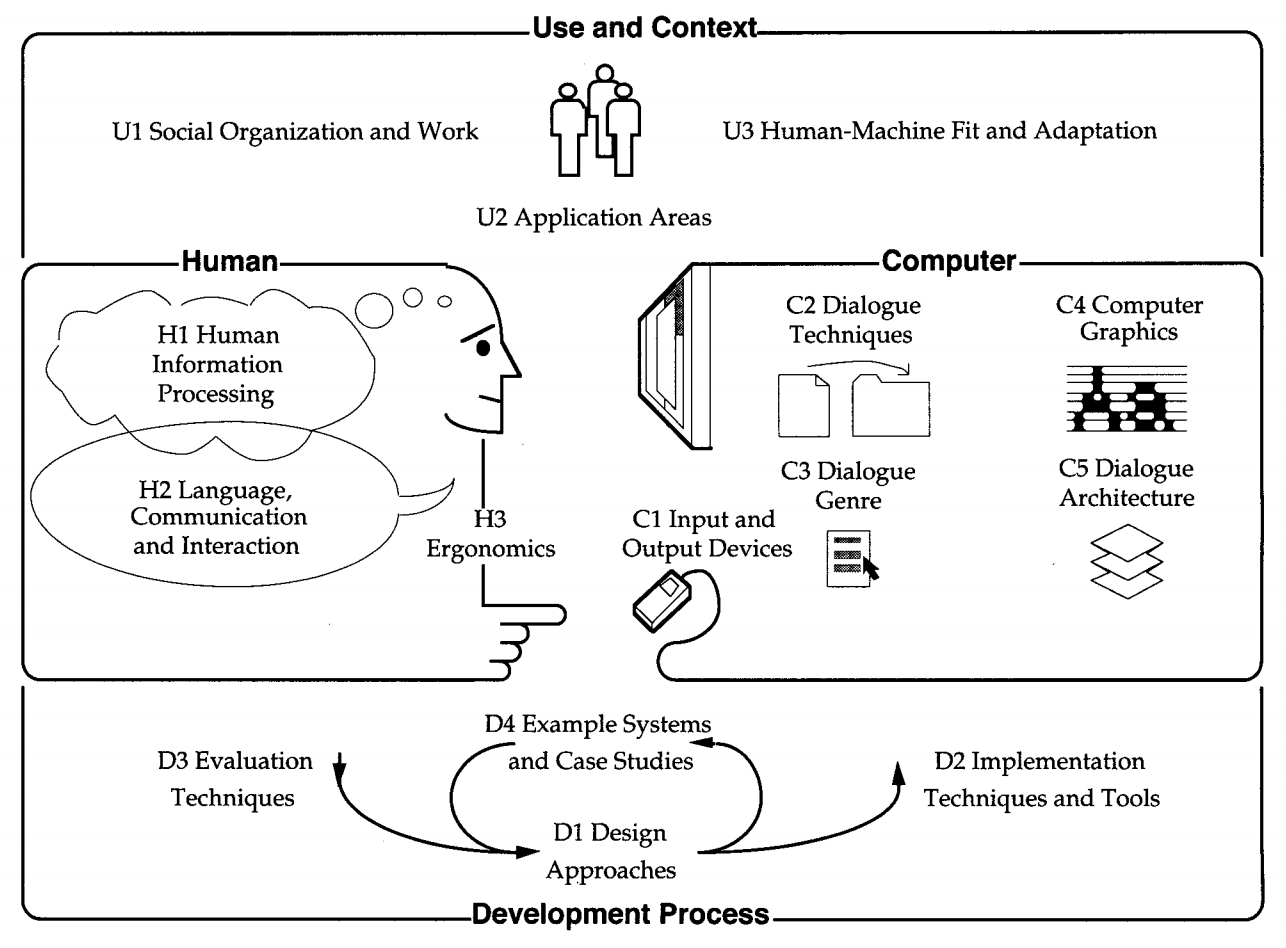
\includegraphics[scale=0.19]{img/content-HCI-1992.png}
\end{figure}
{\small Hewett et al. 1992 \cite{Hewett.1992.curricula}}
\end{frame}
%
\begin{frame}
\frametitle{ACM Classification Keywords}
\begin{quote}
ACM's first classification system for the computing field was published in 1964. Then, in 1982, the ACM published an entirely new system. New versions based on the 1982 system followed, in 1983, 1987, 1991, and 1998. The 2012 scheme utilizes a new poly-hierarchical structure and a more in-depth approach than the 1998 version. It no longer uses the letter-and-number coding of the previous versions. The old scheme has been mapped to the new, and both the 1998 and 2012 terms are available on Citation Pages of all indexed articles in the ACM Digital Library.\\
Source: \url{https://www.acm.org/about-acm/class}
\end{quote}
\end{frame}
%
\begin{frame}
\frametitle{The 2012 ACM Computing Classification System}
\begin{itemize}
\item Hardware
\item Computer Systems Organization
\item Networks
\item Software
\item Theory of Computation
\item Mathematics of Computing
\item Information Systems
\item Security and Privacy
\item Human-Centered Computing
\item Computing Methodologies
\item Applied Computing
\item Social and Professional Topics
\end{itemize}
Source: \url{https://www.acm.org/publications/class-2012-intro}\\
Tool with a visual display: \url{https://dl.acm.org/ccs/ccs.cfm}
\end{frame}
%
\begin{frame}
\frametitle{What is SIGCHI}
ACM SIGCHI is the Special Interest Group  on Human-Computer Interaction.
\begin{quote}
SIGCHI is the premier international society for professionals, academics and students who are interested in human-technology and human-computer interaction (HCI). We provide a forum for the discussion of all aspects of HCI through over 20 sponsored and over 40 in-cooperation conferences, publications (eg. OpenTOC: Table of Contents page), communities, web sites, and other services. We advance education in HCI through workshops and outreach, and we promote informal access to a wide range of individuals and organizations involved in HCI.\\ 
Source: \url{https://sigchi.org/about/about-sigchi/}
\end{quote}
\end{frame}
%
\begin{frame}
\frametitle{How does HCI relate to music tech?}
\begin{quote}
I also discovered that in the grand scheme of things, there are three
levels of design: standard spec, military spec and artist spec. Most significantly,
I learned that the third, artist spec, was the hardest (and most
important). If you could nail it, then everything else was easy. Buxton, 1997 ~\cite{Buxton.1997}
\end{quote}
Lectures 3 and 4 focus on this topic.
\end{frame}
%
\begin{frame}[shrink=20]
\frametitle{How does HCI relate to industry?\\ Technology Innovation Adoption Lifecycle}
\begin{figure}
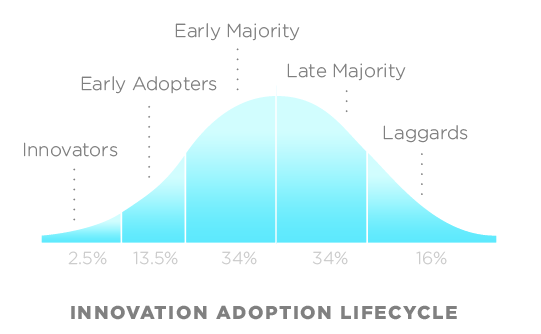
\includegraphics[scale=0.45]{img/DiffusionOfInnovation.png}
\end{figure}
The technology adoption lifecycle is a sociological model that describes the adoption or acceptance of a new product or innovation, according to the demographic and psychological characteristics of defined adopter groups. \\
The process of adoption over time is typically illustrated as a classical normal distribution or ``bell curve''.  \cite{Rogers.1983.diffusion}\\
{\scriptsize Image source: \url{https://en.wikipedia.org/wiki/Technology_adoption_life_cycle}}
\end{frame}

%
%\begin{frame}
%\frametitle{Who are key figures in HCI and why?}
%\begin{itemize}
%\item \end{itemize}
%\end{frame}
%
\begin{frame}
\frametitle{What is CHI?}
\begin{itemize}
{\small
\item CHI stands for the ACM Conference on Human Factors in Computing Systems.
\item The CHI series of academic conferences is generally considered the most prestigious in the field of human-computer interaction and is one of the top ranked conferences in computer science.
\item CHI has been held annually since 1982 and attracts thousands of international attendees. CHI continues to grow, reaching over 3,300 attendees in 2013 and 3,800 in 2016.
\item Since 1993 the acceptance rate for full papers was consistently below 30 percent. After 1992 the average acceptance rate was around 20 percent. The number of accepted full papers is slowly increasing and reached 157 accepted papers with an acceptance rate of 22 percent in 2008.
\item The Proceedings of CHI can be found on the ACM Digital Library: \url{https://dl.acm.org/}
}
\end{itemize}
{\scriptsize Source: \url{https://en.wikipedia.org/wiki/Conference_on_Human_Factors_in_Computing_Systems}}
\end{frame}
%
\begin{frame}
\frametitle{When Second Wave HCI meets Third Wave Challenges}
\begin{quote}
Abstract: This paper surveys the current status of second generation HCI theory, faced with the 
challenges brought to HCI by the so-called third wave. In the third wave, the use context and application types are broadened, and intermixed, relative to the focus of the second wave on work. Technology spreads from the workplace to our homes and everyday lives and culture. Using these challenges the paper specifically addresses the topics of multiplicity, context, boundaries, experience and participation in order to discuss where second wave theory and conceptions can still be positioned to make a contribution as part of the maturing of our handling of the challenges brought on by the third wave. \\
B{\o}dker, 2006 \cite{Bodker.2006.second}
\end{quote}
\end{frame}
%
\begin{frame}
\frametitle{The `third wave'}
The `third wave' provides a different lens for understanding alternative computing systems to window-icon-mouse-pointer systems, such as ubiquitous, mobile, collaborative or social computing systems. This paradigm is referred by~\cite{Harrison.et.al.2007.three} as `situated perspectives', a sum of perspectives that studies HCI interaction as situated in a particular context and which connects to qualitative disciplines such as ethnography or practice-based research.
\end{frame}
%
\begin{frame}
\frametitle{The three paradigms compared}
\begin{figure}
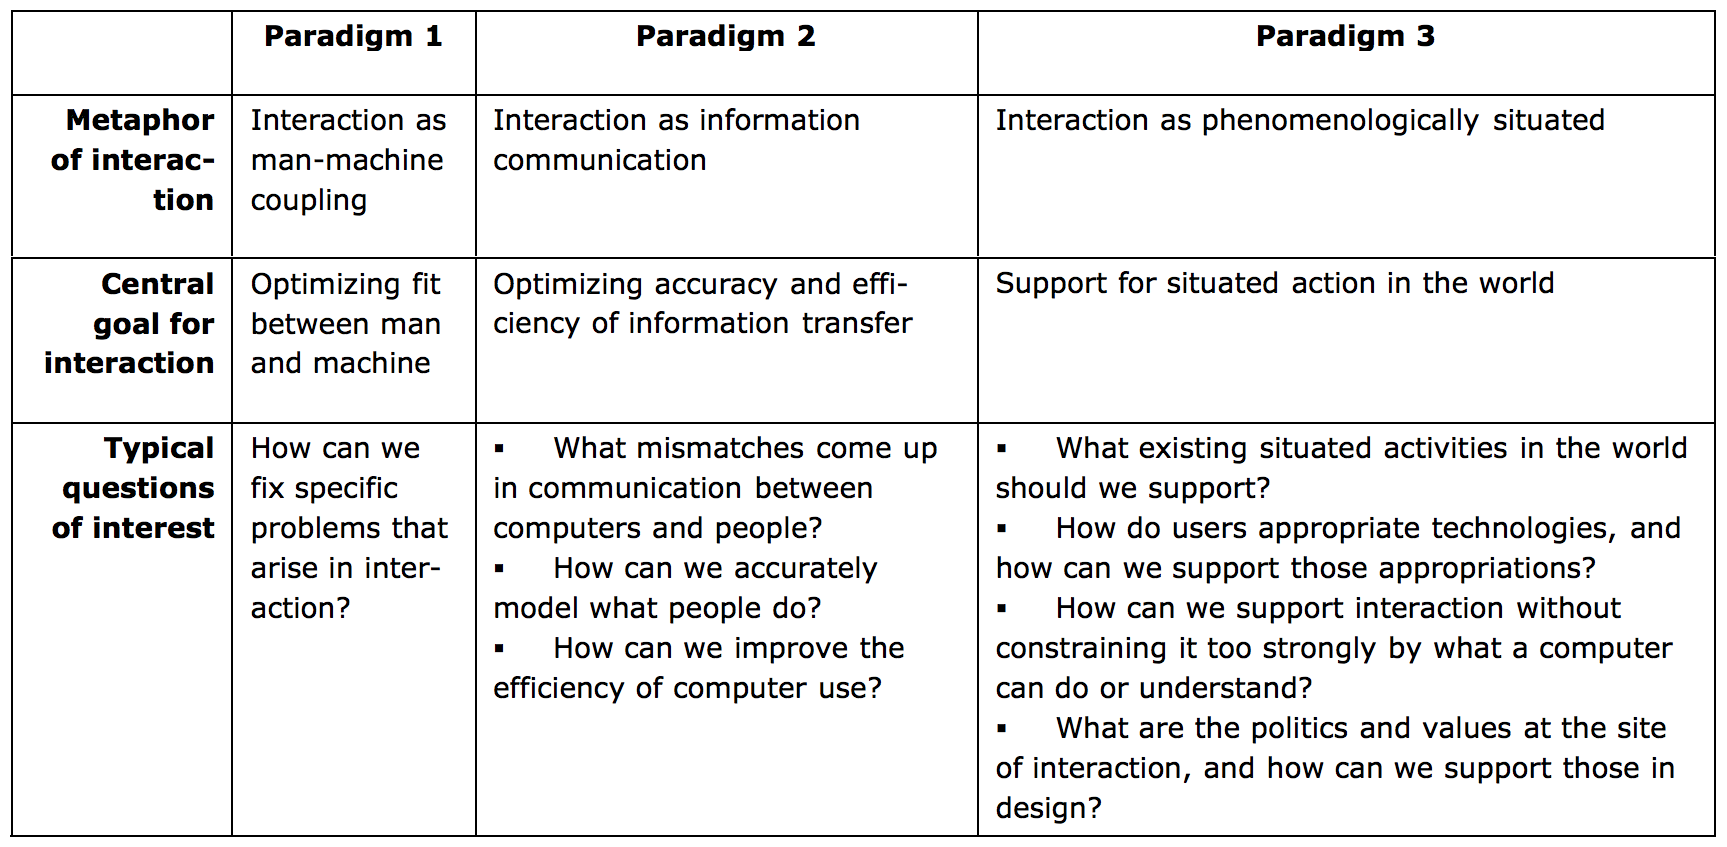
\includegraphics[scale=0.18]{img/the-three-HCI-paradigms.png}
\end{figure}
{\scriptsize Harrison et al. (2007) \cite{Harrison.et.al.2007.three}}
\end{frame}
%
\begin{frame}
\frametitle{Third-Wave HCI, Ten Years Later (B{\o}dker, 2015)}
{\small
\begin{itemize}
\item The first wave was cognitive science and human factors. It was model-driven and focused on the human being as a subject to be studied through rigid guidelines, formal methods, and systematic testing. \cite{Bodker.2015.third}
\item The second wave is the move ``from human factors to human actors.'' In the second wave, the focus was on groups working with a collection of applications. Focus on situated action, distributed cognition, context, and proactive methods (e.g. participatory design, prototyping). \cite{Bodker.2015.third}
%Theory focused on work settings and interaction within well-established communities of practice. Situated action, distributed cognition, and activity theory were important sources of theoretical reflection, and concepts like context came into focus in the analysis and design of human-computer interaction. Proactive methods, such as a variety of participatory design workshops, prototyping, and contextual inquiries, were added to the toolbox. 
\item  In the third wave, technology spread from the workplace to our homes and everyday lives and culture. Focus on understanding experience and meaning-making. \cite{Bodker.2015.third}
\end{itemize}
}
\end{frame}
%
\begin{frame}
\frametitle{Examples}
{\small
\begin{itemize}
\item \emph{Example first wave}\\ Fitts's Law: \url{https://www.interaction-design.org/literature/book/the-glossary-of-human-computer-interaction/fitts-s-law}
\item \emph{Example second wave}\\ Distributed Cognition in an Airline Cockpit: \url{http://hci.ucsd.edu/media/uploads/hci_papers/EH1996-1.pdf} \cite{Hutchins.Klausen.1996.distributed}
\item \emph{Example third wave}\\ Where The Action Is: The Foundations of Embodied Interaction by Paul Dourish: \url{https://www.dourish.com/embodied/} \cite{Dourish.2004.embodiedinteraction}
\end{itemize}
}
\end{frame}
%
\begin{frame}
\frametitle{What is NordCHI?}
\begin{quote}
NordiCHI is a biennial conference functioning as the main Nordic forum for human-computer interaction research. NordiCHI is the meeting place for researchers from academia and industry, designers, practitioners, educators and others from a broad range of traditions and communities. The NordiCHI conference takes HCI in the non-limited sense of research and practice addressing the design and use of interactive technology. The NordiCHI conference is a joint effort initiated by Nordic HCI organisations (some of which do not exist anymore).  \\
\url{https://www.nordichi.eu/}
\end{quote}
\end{frame}
%
\begin{frame}
\frametitle{}
\Huge{Roadmap: Being Human}
\end{frame}
%
\begin{frame}
\frametitle{Being human: HCI in the year 2020}
\begin{quote}Computer technologies are not neutral -- they are laden with human, cultural and social values.  We need to define a new agenda for human-computer interaction in the 21st century --- one that anticipates and shapes the impact of technology rather than simply reacts to it. \\
{\scriptsize Source: \url{https://hxd.research.microsoft.com/work/being-human-human-computer-interaction-in-the-year-2020.php} }
\end{quote}
\begin{itemize}
\item What is a roadmap or agenda?
\item After 10 years of the publication of this agenda, to what extent their predictions have been successful or not. Any surprises?
\end{itemize}
\end{frame}
%
\begin{frame}
\frametitle{Being human: HCI in the year 2020: Discussion}
 \begin{figure}
	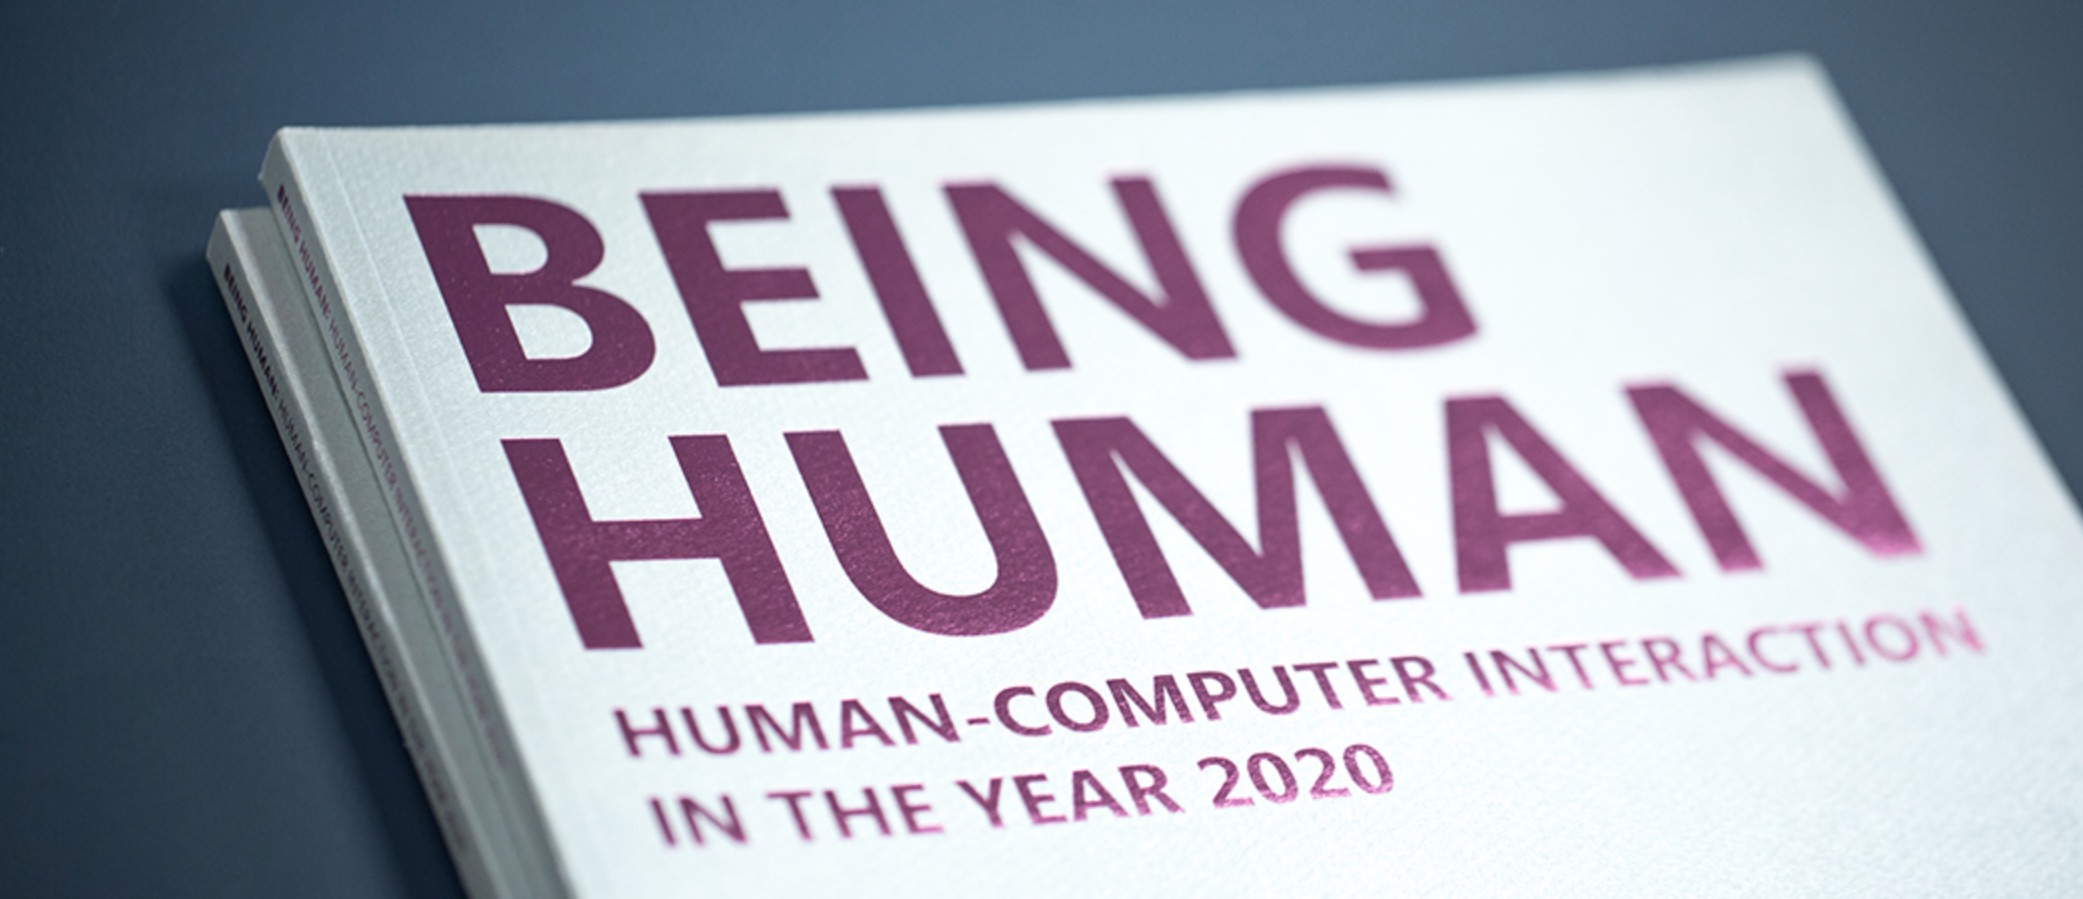
\includegraphics[scale=0.12]{img/being-human.jpg}
    \end{figure}	
\begin{itemize}
\item 10.30-11.00 Discussion about the prep. reading framed in the context of the three waves in HCI.
\end{itemize}
\end{frame}
%
\begin{frame}
\frametitle{CHI 2019 Best Papers}
\begin{itemize}
\item 11.00-11.30 Teamwork: Selection of a paper from the CHI 2019 Best Papers (\url{https://chi2019.acm.org/2019/03/15/chi-2019-best-papers-honourable-mentions/}) and discussion about what is the research question, the approach used to address the research question, the main findings and the main contribution.
\item 11.30-12.00 The teams summarize to the group their selected paper (10 min per group).
\end{itemize}
\end{frame}
%
\begin{frame}
\frametitle{Final Remarks (1/3)}
\begin{itemize}
\item In the 21st century, sophisticated information and communication technologies are emerging different from the 20th century, and bringing different opportunities and challenges.
\item At the same time, engineering, humanities and artistic subjects are all relevant in order to tackle the increasingly complex modern technical society. 
\end{itemize}
\end{frame}
%
\begin{frame}
\frametitle{Final Remarks (2/3)}
``Renaissance thinking'' in modern HCI \cite[p.196]{Gross.2014:ICHCI} as so well represented by Leonardo da Vinci and as pointed out by Shneiderman \cite[p.2--3]{Shneiderman.2003:MITPress}:
\begin{quote}
\emph{This modern Renaissance would unify thinking about technology by promoting multidisciplinary education and a sympathy for diversity. [ \ldots ] However, linking the high-tech world more closely to the needs of people still requires some new forms of thinking. The Renaissance integration of disciplines that Leonardo da Vinci exemplified could guide us in repairing the split in our modern world. }
\end{quote}
\end{frame}
%
\begin{frame}
\frametitle{Final Remarks (3/3)}
\begin{itemize}
\item HCI is an important subject to be taught in courses related to prototyping interactive computer-based systems and can provide a theoretical framework and critical thinking tool to support building new technology.
\item TBL is a suitable pedagogical method to teach HCI in future educational scenarios due to the promotion of teamworking within diverse complementary teams and for problem-solving societal challenges.
\item Being technological humanists means being responsible thinkers and makers. 
\end{itemize}
\end{frame}
%
\begin{frame}
\frametitle{Human-Computer Interaction Day 1 - Group Assignment (post-class)}
\begin{itemize}
\item Send a summary (1 page max.) of the selected article discussed in group during class from the CHI 2019 Best Papers after the class on Tuesday 22 October 2019 and before Thursday 24 October 2019 9:00. 
You should explain the research question, the approach used to address the research question, the main findings and the main contribution and include the feedback from the class.
\end{itemize}
\end{frame}
%
\begin{frame}
\frametitle{Human-Computer Interaction Day 2 - Individual Assignment}
\begin{itemize}
\item Send a summary (1 page max.) of the following article before Thursday 24 October 2019 9:00 and be ready to discuss it in class:\\ 
From Mice to Men - 24 years of Evaluation in CHI~\cite{Barkhuus.Rode.2007.evalchi}\\
The summary should include: 
the main topic of the paper,
the research question,
the approach used to address the research question,
the main findings, and
the main contribution.
\end{itemize}
\end{frame}
%
\begin{frame}
\frametitle{Resources}
\begin{itemize}
\item SIGCHI: \url{https://sigchi.org/}
\item HCI Bibliography: \url{http://www.hcibib.org/}
\item HCI Glossary - Alan Dix: \url{https://alandix.com/academic/papers/theory-formal-2003/glossary.html}
\item The Glossary of Human Computer Interaction: \url{https://www.interaction-design.org/literature/book/the-glossary-of-human-computer-interaction}
\end{itemize}
\end{frame}
%
\begin{frame}[shrink=20]
  \frametitle{References}
  \printbibliography
\end{frame}
%
\end{document}
